%%%%% --------------------------------------------------------------------------------
%%
%%                               Document Template
%%
%%%%% --------------------------------------------------------------------------------
%% Copyright (C) 2014-2018 Huangrui Mo <huangrui.mo@gmail.com> 
%% This is free software: you can redistribute it and/or modify it
%% under the terms of the GNU General Public License as published by
%% the Free Software Foundation, either version 3 of the License, or
%% (at your option) any later version.
%%%%% --------------------------------------------------------------------------------
%%
%%%%*************************Document Class Declaration*******************************
%%
\documentclass[doublesided]{uwaterloothesis}% thesis template of University of Waterloo
%% Multiple optional arguments:
%% [<singlesided|doublesided|printcopy>] % single-sided, double-sided, or print layout 
%% [draftversion] % show draft version information, default is no show
%% [standard options for book class]
%%%%% --------------------------------------------------------------------------------
%%
%%%%**************************Command Define and Settings*****************************
%%
\usepackage{commons}% common settings
%% usage: \usepackage[option1,option2,...,optionN]{commons}
%% Multiple optional arguments:
%% [<numbered|authoryear|alpha>] % citation and reference style
%% <numbered>: textual: Jones [1]; parenthetical: [1]. default style
%% <authoryear>: textual: Jones (1995); parenthetical: (Jones, 1995)
%% <alpha>: textual: not available; parenthetical: [Jon95]
%% [myhdr] % one available header and footer style, will enable fancyhdr
%% [lscape] % provide landscape layout environment
%% [geometry] % configure page layout by geometry package
%% [list] % enable enhanced list environments, useful for Algorithm and Coding
%% [color] % enable color package to use color, current package is xcolor
%% [background] % enable page background, will auto enable color package
%% [tikz] % enable tikz for complex diagrams, will auto enbale color package
%% [table] % enable a table package for complex tables, current is ctable
\usepackage{custom}% user defined commands
%%%%% --------------------------------------------------------------------------------
%%
%%%%*********************************Content******************************************
%%
\begin{document}
%%
%%%%% --------------------------------------------------------------------------------
%%
%%%%*********************************Frontmatter**************************************
%%
%% Frontmatter of Title page, Table of contents, Preface chapter.
\frontmatter
%%
%% >>> Frontpages
%%
%%
%% >>> Title Page
%%
%%\LaTeX{} is Latex printed in right way
%% Define new commands (add space after defined names0
\newcommand{\Company}{Altaeros Energies }
\newcommand{\Term}{3B }
\newcommand{\Seb}{Sebastien Blanchet }
\newcommand{\ReportTitle}{Numerical Analysis of Externally Pressurized Cylinder}
\newcommand{\CompanyCity}{Somerville, Massachusetts, United States}

\newcommand*{\SignatureAndDate}[1]{%
    \par\noindent\makebox[2.5in]{\hrulefill} \hfill\makebox[2.0in]{\hrulefill}%
    \par\noindent\makebox[2.5in][l]{#1}      \hfill\makebox[2.0in][l]{Date}%
}

%% Define command variable names
\title[WKRPT 400]{WKRPT 400\\ \ReportTitle}% \title[short title for headers]{Long title of thesis}
\author{\Seb}
\preparedfor{\Company}
\preparedcity{\CompanyCity}
\discipline{\Term Mechanical Engineering}
%make title page
\maketitle


%%
%% >>> author's declaration
%%
\begin{declaration}

	\Company\\
	24 Park Street, Unit 10\\
	\CompanyCity , 02143\\
	\\ 
    Professor Michael Collins\\
	Associate Chair Undergraduate Studies, Mechanical Engineering\\
	University of Waterloo\\
	Waterloo, Ontario, Canada, N2L 3G1\\
	\\ 
    Dear Professor Collins,\\ 
    \\
    Prepared for my \Term work term at \textbf{\textsl{\Company}}, my third and final work term report is
	entitled \textbf{\textsl{\ReportTitle}}. The objective of this work term report was to perform an in depth structural analysis on the current aerostat's winch system.\\ 
	\\
	\Company  has one simple mission, to deliver telecommunication in remote areas with increased reliability and more cost effectively. Another major selling point is fully autonomy led by state of the art controls.\\
	\\
	As a systems engineering intern under the supervision of Ephraim Lanford, I was primarily responsible for conducting advanced analyses on the aerostat's tether management system.\\ 
	\\
	This report was written entirely by me and has not received any previous academic credit at this or
	any other institution. I would like to thank Ephraim Lanford for all guidance. Also, John Umina for his expertise in the design of pressure vessels. No other sources of aid were used for this report.\\ 
	\\
	Best Regards,\\
	\\
	\Seb\\
	%Hide ID num, write it when signing report
	ID: \\
	%% Create signature line and date before handing in
	\Term Mechanical Engineering\\
	\SignatureAndDate{Signature}
	
	% Hide page num
	\thispagestyle{empty}
	
\end{declaration}


%%
%% >>> abstract
%%
%\intotoc{Abstract}% add a corresponding item to the contents table and bookmark
%\begin{abstract}
%
%	\noindent
%	The objective of this report is \\
%	\\
%	Preliminary results found that the method was not good.\\ 
%	\\
%	Results\\
%	\\
%	Conclusions and recommendations\\
%\end{abstract}


%%
%%% >>> List of Content
%%
\tableofcontents% contents catalog
\listoftables% tables catalog
\intotoc{List of Tables}% add a corresponding item to the contents table and bookmark
\listoffigures% figures catalog
\intotoc{List of Figures}% add a corresponding item to the contents table and bookmark
%%
%% >>> prematter
%%
%
% >>> Nomenclatures
%
\chapter{Glossary}
%% Symbols
\nomenclatureitem[\textbf{Unit (SI)}]{\textbf{Symbol}}{\textbf{Description}}
\nomenclatureitem[$\Unit{mm}$]{$a$}{Cylindrical Shell Radius}
\nomenclatureitem[$\Unit{mm}$]{$d$}{Tether Diameter}
\nomenclatureitem[$\Unit{mm}$]{$D$}{Outer Drum Diameter}
\nomenclatureitem[$\Unit{GPa}$]{$E$}{Young's Modulus}
\nomenclatureitem[$\Unit{mm}$]{$h$}{Cylindrical Thickness}
\nomenclatureitem[$\Unit{mm^4}$]{$I$}{Moment of Inertia}
\nomenclatureitem[$\Unit{mm}$]{$L$}{Drum Length}
\nomenclatureitem[$\Unit{MPa}$]{$L'$}{Critical Buckling Length}
\nomenclatureitem[$\Unit{-}$]{$n$}{Safety Factor}
\nomenclatureitem[$\Unit{N}$]{$N$}{Normal Force}
\nomenclatureitem[$\Unit{N \cdot mm}$]{$M$}{Moment}
\nomenclatureitem[$\Unit{MPa}$]{$p$}{Pressure}
\nomenclatureitem[$\Unit{MPa}$]{$p'$}{Critical Buckling Pressure}
\nomenclatureitem[$\Unit{mm}$]{$R$}{Outer Drum Radius}
\nomenclatureitem[$\Unit{mm}$]{$t$}{Thickness}
\nomenclatureitem[$\Unit{N}$]{$T$}{Tether Tension}
\nomenclatureitem[$\Unit{mm}$]{$u$}{$x$ Displacement}
\nomenclatureitem[$\Unit{N}$]{$V$}{Shear Force}
\nomenclatureitem[$\Unit{mm}$]{$w$}{$z$ Displacement}
%Greek
\nomenclatureitem[$\Unit{-}$]{$\beta$}{Thin Shell Parameter}
\nomenclatureitem[$\Unit{-}$]{$\varepsilon$}{Strain}
\nomenclatureitem[$\Unit{Radians}$]{$\theta$}{Contact Angle}
\nomenclatureitem[$\Unit{-}$]{$\lambda$}{Load Factor}
\nomenclatureitem[$\Unit{-}$]{$\mu$}{Coefficient of Static Friction}
\nomenclatureitem[$\Unit{-}$]{$\nu$}{Poisson's Ratio}
\nomenclatureitem[$\Unit{MPa}$]{$\sigma$}{Stress}
\nomenclatureitem[$\Unit{MPa}$]{$\sigma_a$}{Allowable Stress}
\nomenclatureitem[$\Unit{MPa}$]{$\sigma_h$}{Hoop Stress}
\nomenclatureitem[$\Unit{MPa}$]{$\sigma_y$}{Yield Strength}
\nomenclatureitem[$\Unit{Radians}$]{$\varphi$}{Differential Angle}
\nomenclatureitem[$\Unit{-}$]{$\psi$}{Buckling Mode}
\nomenclatureitem[]{}{}

%% Acronym
\nomenclatureitem{\textbf{Acronym}}{\textbf{Description}}
\nomenclatureitem{ASME}{American Society of Mechanical Engineers}
\nomenclatureitem{BC}{Boundary Conditions}
\nomenclatureitem{BPVC}{Boiler and Pressure Vessel Code}
\nomenclatureitem{DNV}{Det Norske Veritas}
\nomenclatureitem{FEA}{Finite Element Analysis}
\nomenclatureitem{ID}{Inner Diameter}
\nomenclatureitem{OD}{Outer Diameter}
\nomenclatureitem{ODE}{Ordinary Differential Equation}
\nomenclatureitem{SF}{Safety Factor}
\nomenclatureitem{SI}{International System of Units}
\nomenclatureitem{TMS}{Tether Management System}
\nomenclatureitem{TWPV}{Thin Walled Pressure Vessel}
\nomenclatureitem{USC}{United States Customary}


%% >>> Summary
%%
\chapter{Summary}

The objective of this report is to perform a structural analysis on Altaeros' grounded TMS winch, focusing on the sizing of drum and flange thicknesses.\\

An external pressure $p=1376\Unit{psi}= 9.486\Unit{MPa}$ is calculated from the Capstan equation as a result of the tethers tension. Initial drum thicknesses are determined by study of ASME's BPVC, EN, DNV and TWPV standards yielding a range of $t\in [0.825, 1.680]$ in / $\in [21.0, 43.2]$ mm.\\

The thin shell theory is presented to setup analytical results of fixed end cylinder loaded with uniform pressure $p$ yielding a drum thickness of 1.686 in / 42.8 mm. Buckling analysis is also completed, resulting in 0.418 in / 10.6 mm for a critical buckling pressure of $p'=p$, confirming that buckling is not the primary mode of failure.\\

%%%%%
A series of ANSYS FEA simulations were completed to understand the equivalent stresses for various loading scenarios (focus on USC units). Run 1 explored uniform pressure $p$ with both fixed and simply supported ends yielding required thicknesses of 1.200 \& 0.875 in respectively. Run 2 focused on modeling the exponential decay as per Capstan equation with fixed and simply supported ends yielding 0.650 \& 0.550, respectively. Run 3 focused on a linear eigenvalue buckling analysis to confirm analytical findings. A critical thickness of 0.375 in was yielded. Run 4 served as a preliminary benchmark for flange design. An optimal flange thickness is 0.250 in was observed.\\

In summary, the drum barrel shall be manufactured with a Schedule 30 ($t=$ 0.625 in), 28 in OD pipe. Flanges should be cut from a $3\Unit{feet}^2$ by $0.250\Unit{in}$ thick plate.\\

Future work should focus on flange design, non linear buckling, fatigue analysis and proof testing.% list of symbols, preface of books
%%
%%%%% --------------------------------------------------------------------------------
%%
%%%%*********************************Mainmatter***************************************
%%
%% Main topics.
\mainmatter
%%
%%% >>> Main Contents
%%
%%%%% --------------------------------------------------------------------------------
%%
%%%%********************************Main Content**************************************
%%
%%% ++++++++++++++++++++++++++++++++++++++++++++++++++++++++++++++++++++++++++++++++++
%\renewcommand{\chaptername}{Section}

%-----------------------------------------------------------------------------------------------------------------
%% Section 1 : Introduction
\chapter{Introduction}
\label{chapt:intro}

This is the introduction, why we are doing this analysis

\section{Background} % (fold)

\Company does this as per Figure~\ref{fig:companypic} seen below.

%% REFERENCE:
%%[htbp] (here, top, bottom, page).  ! means no restriction for placement
%%http://tex.stackexchange.com/questions/2275/keeping-tables-figures-close-to-where-they-are-mentioned help
\begin{figure}[!htbp]
    \centering
    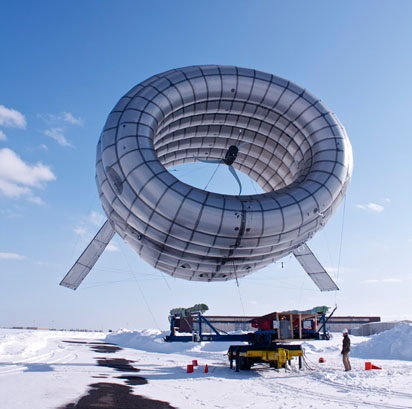
\includegraphics[width=0.6\textwidth]{companypic}
    \caption{Overview of the buoyant airborne technology}
    \label{fig:companypic}
\end{figure}


\section{Purpose}
The purpose of this report is to do this.
\begin{itemize}
    \item Do analysis on drum
    \item Development numerical algorithm for solving
\end{itemize}


\section{Scope} % (fold)

The scope of the report will be as follows.


%-----------------------------------------------------------------------------------------------------------------
%% Section 2 : Preliminary Analysis
\chapter{Preliminary Analysis}
\label{chapt:prelim}

The analysis process is discussed

\section{Simplifications}

The results were simplified to do.

%Example of using an equation and refering to it
\subsection{Equations}


The first equation that is presented , Equation~\ref{eq:eqnstatics}

% First equation of basic statics
\begin{equation}
\label{eq:eqnstatics}
	% must use aligned to get multi line equation	
	\begin{aligned}
		\Sigma F_i=0\\
		\Sigma M_i=0
	\end{aligned}
\end{equation}


As per reference \cite{timoshenko1959theory}

%Example of using table
\subsection{Table}

This was used to get the results in the following Table~\ref{table:testtbl}.
	
	\begin{table}[ht]
		\caption{Test table 1}
		\centering
		\begin{tabular}{c c c}
			%heading
			\hline \hline  Case & Method \#1 & Method \#2 \\[0.5ex]
			\hline
			%Main table body content	
			1 & 10 & 50\\
			2 & 20 & 100\\ [1ex]
			\hline
		\end{tabular}
		\label{table:testtbl}
	\end{table}

\section{Theory of Cylindrical Shells}

As per Timoshenko's book, this section will cover the method of approximating the cylinder as a long thin shell.

%-----------------------------------------------------------------------------------------------------------------
%% Section X : Discussion
\chapter{Discussion}

%-----------------------------------------------------------------------------------------------------------------
%% Section X : Conclusion
\chapter{Conclusion}

%-----------------------------------------------------------------------------------------------------------------
%% Section X : Reccomendations
\chapter{Recommendations}

%-----------------------------------------------------------------------------------------------------------------
%% Section X : As per template 
\chapter{Supplemental}
\subsection{Installation} % (fold)
\LaTeX is based on open-source code, so it is available on most computing platforms as free software. If encounter some compiling problems after installation, please Google it. For example, MikTeX may complain about "mathtools.sty", a solution given on "StackExchange" is "The problem is that the package manager has somehow "desynchronized" (even though it's a fresh install). To fix it, run Miktex Package Manager as administrator---"Package Manager (Admin)". Go to Repository--Synchronize. When that completes, your TexWorks should automatically find the needed style files again."
\begin{itemize}
    \item Linux: TeXLive distribution. 
    \item MacOS: Mactex or TeXLive.
    \item Windows: MikTeX or TeXLive. 
\end{itemize}

Note: to use \LaTeX{}, you need a text editor for writing and editing ".tex" files. To open the ".tex" files in this template, you need a text editor which supports "UTF-8" encoding. Free options for different platforms are the following:
\begin{itemize}
    \item Linux: vim. 
    \item MacOS: TeXShop, Macvim.
    \item Windows: Texmaker, Gvim, Notepad++. 
\end{itemize}
% subsection Installation (end)

\subsection{Give a try} % (fold)
After downloading this template and installing a \LaTeX{} distribution. It's time to have a try:
\begin{itemize}
    \item Linux: run Compile.sh
    \item MacOS: run Compile.sh
    \item Windows: run Compile.bat
\end{itemize}

% subsection Give a try (end)

\subsection{Include math} % (fold)
\LaTeX{} realization of Equation~\ref{eq:N-S_equation} is something like this:
\begin{center}
    \small
    % Verbatim is used to show the actual latex comands and not complied
    \begin{verbatim}
    \begin{equationa}\label{eq:N-S_equation}
        \frac{\partial (\rho\mathbf{v})}{\partial t} +
        \nabla \cdot (\rho \mathbf{v} \mathbf{v}) =
        -\nabla p + \nabla \cdot\mathbf{T} + \mathbf{f}. 
    \end{equation}    
\end{verbatim}
\end{center}

\begin{equation}\label{eq:N-S_equation}
    \frac{\partial (\rho\mathbf{v})}{\partial t} + \nabla \cdot (\rho \mathbf{v} \mathbf{v}) = -\nabla p + \nabla \cdot\mathbf{T} + \mathbf{f}. 
\end{equation}    
% subsection Include math (end)

\subsection{Include Graphics} % (fold)
Note: inluding figures may seem to be scary by looking at the codes. However, the fact is that you only need to modify the names in each part, the rest are simply copy and paste. These codes are all available in the file "Useful Commands.txt".

Figure~\ref{fig:ITC_Q_Criteria} is an example for including a single figure.
\begin{center}
    \small
    \begin{verbatim}
        \begin{figure}[!htbp]
            \centering
            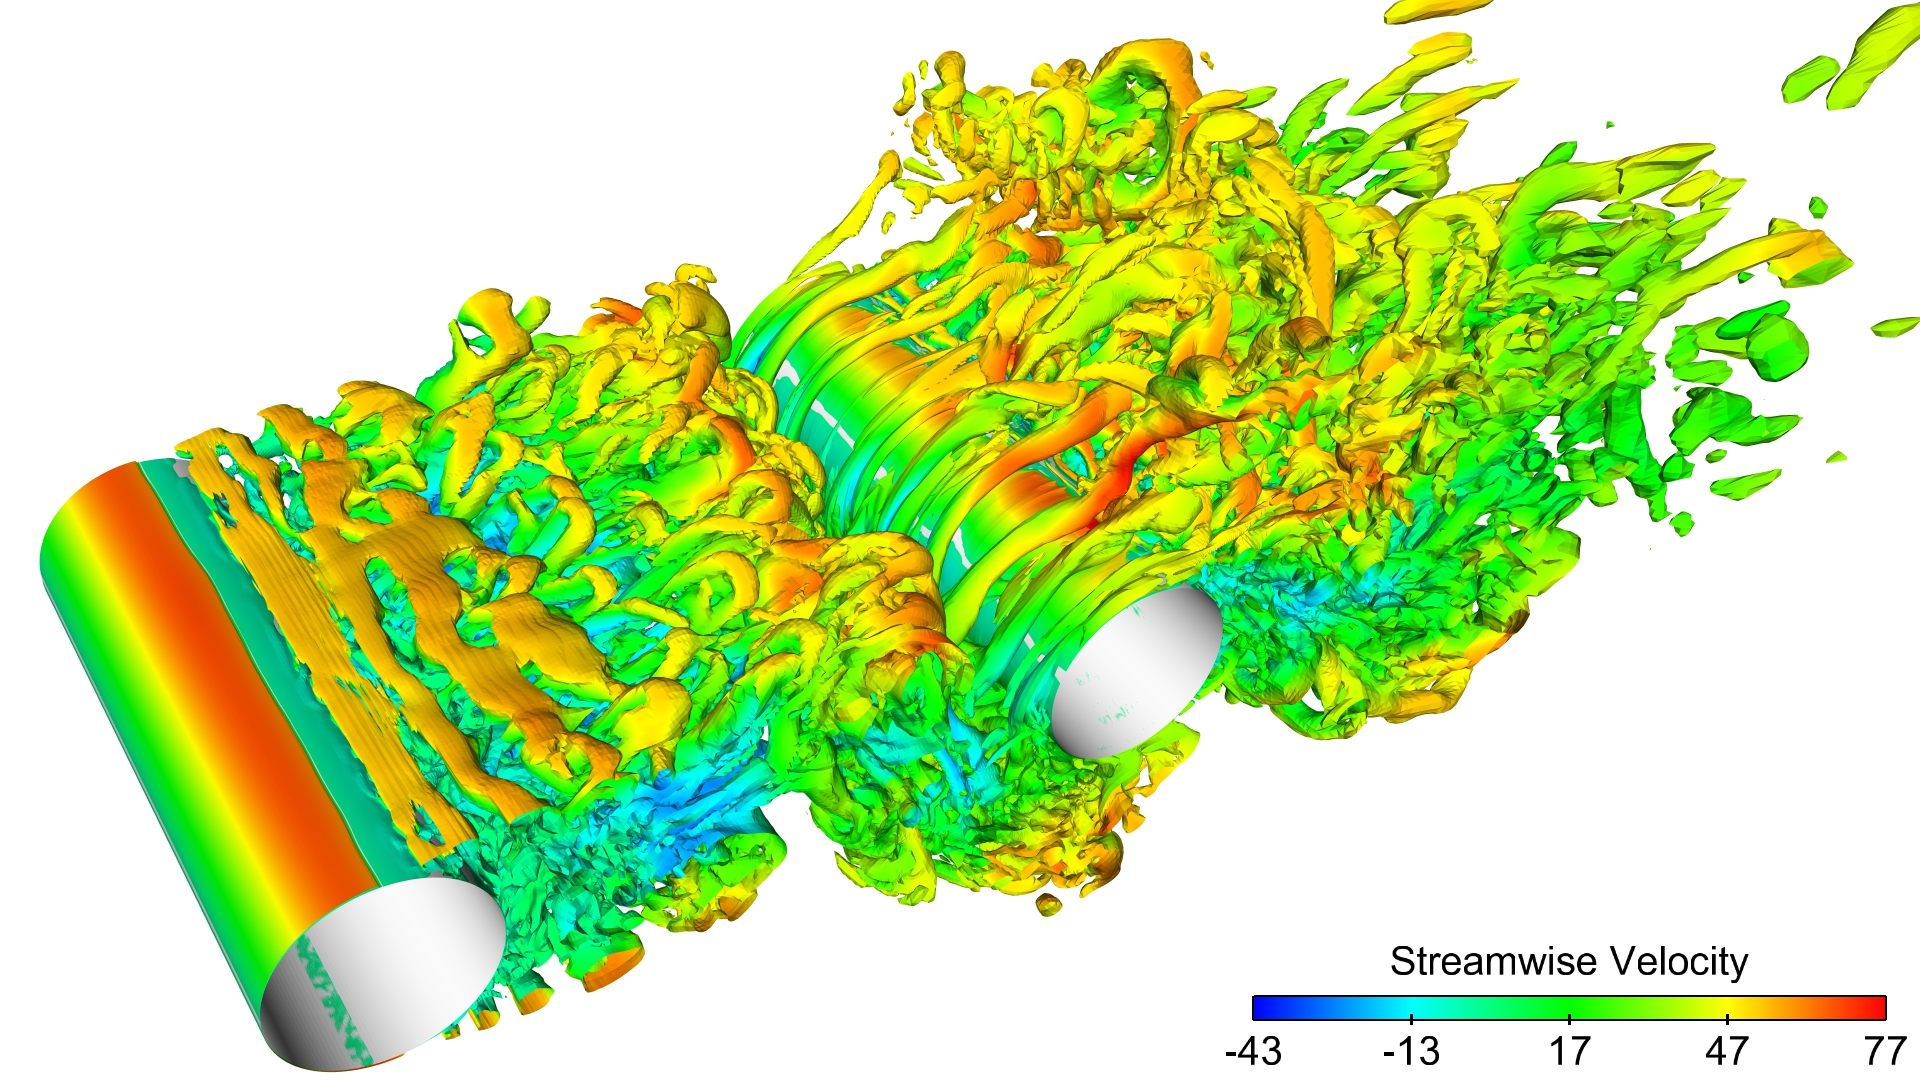
\includegraphics[width=0.45\textwidth]{ITC_Q_Criteria}
            \caption{An Example for including a single figure}
            \label{fig:ITC_Q_Criteria}
        \end{figure}
    \end{verbatim}
\end{center}

\begin{figure}[!htbp]
    \centering
    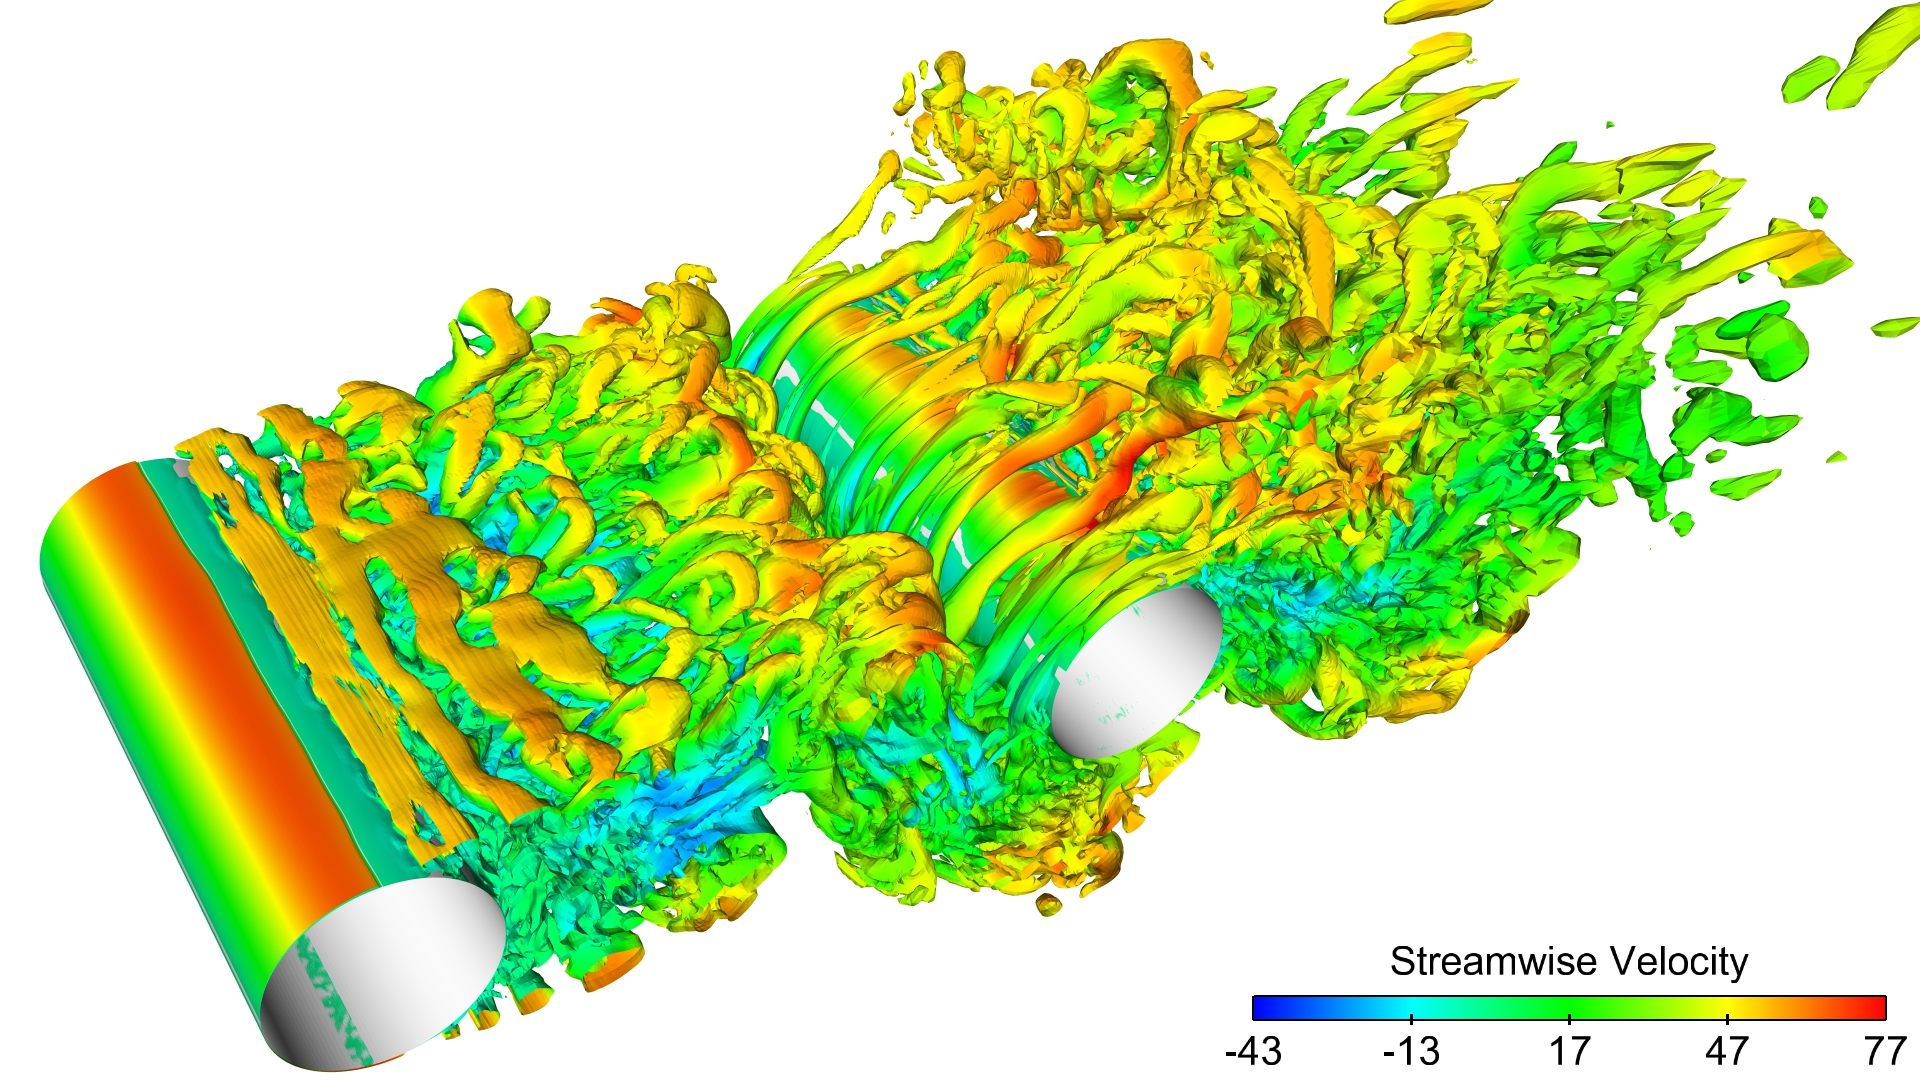
\includegraphics[width=0.45\textwidth]{ITC_Q_Criteria}
    \caption{An Example for including a single graph}
    \label{fig:ITC_Q_Criteria}
\end{figure}

Figure~\ref{fig:HC_OASPL} is an example for including multiple figuress. 
\begin{center}
    \small
    \begin{verbatim}
        \begin{figure}[!htbp]
            \centering
            \begin{subfigure}[b]{0.45\textwidth}
                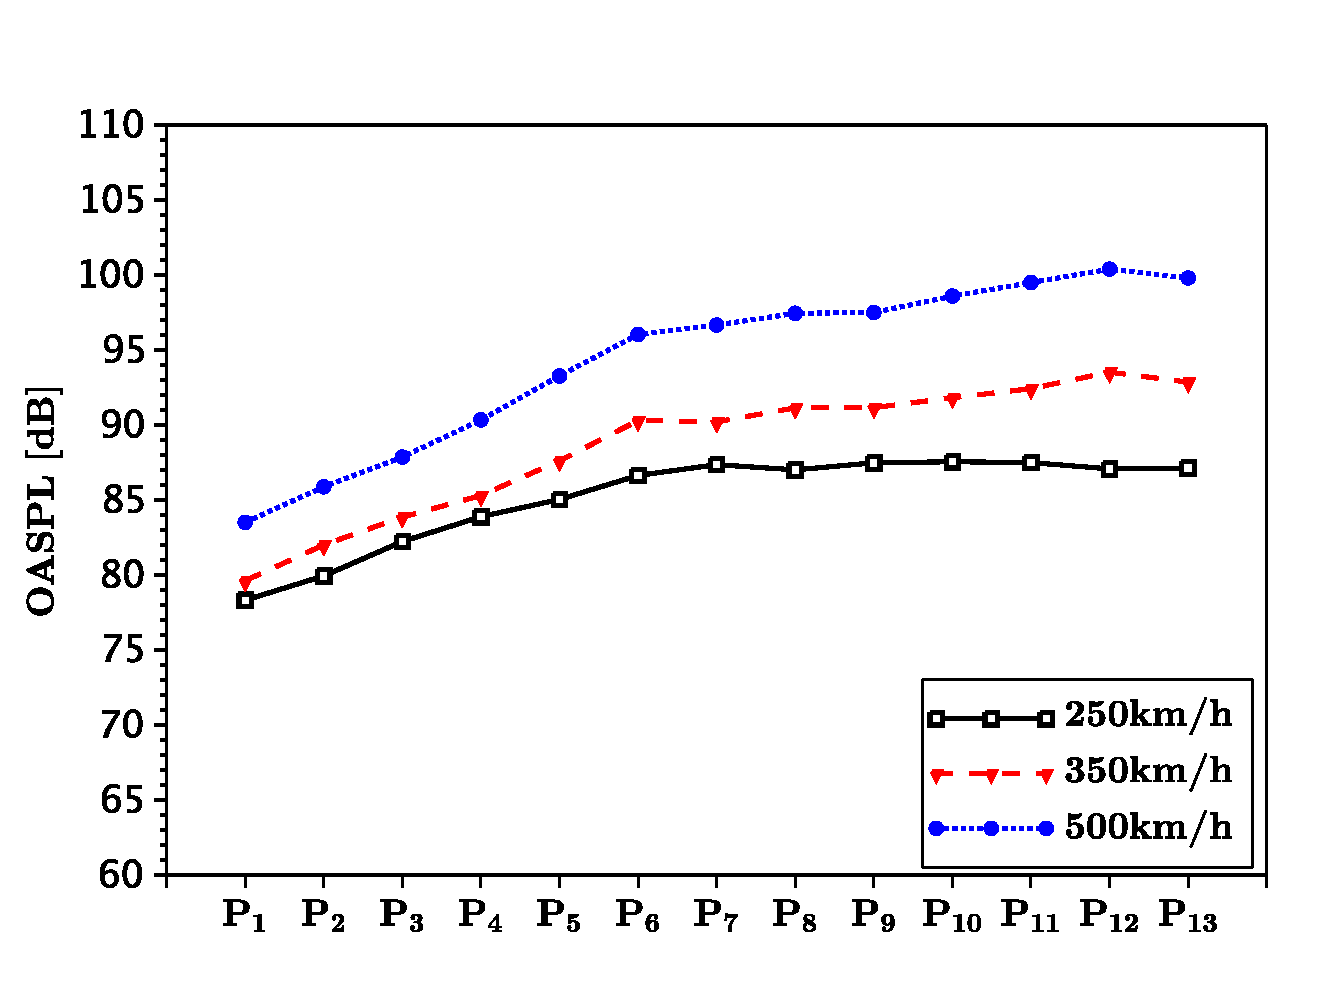
\includegraphics[width=\textwidth]{HC_OASPL_A}
                \caption{}
                \label{fig:HC_OASPL_A}
            \end{subfigure}%
            ~% add a small space
            \begin{subfigure}[b]{0.45\textwidth}
                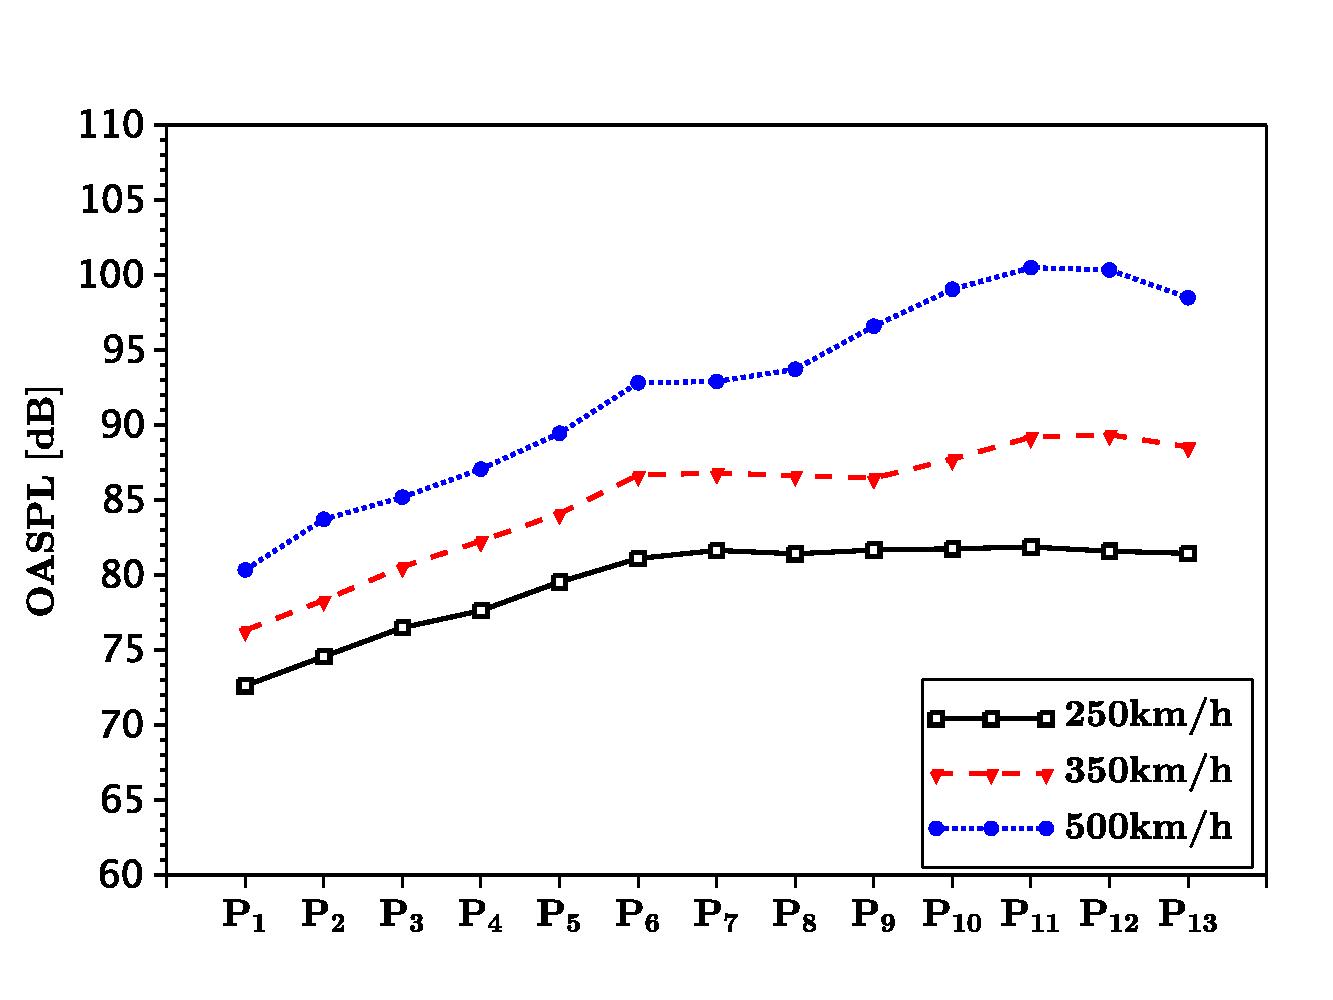
\includegraphics[width=\textwidth]{HC_OASPL_B}
                \caption{}
                \label{fig:HC_OASPL_B}
            \end{subfigure}%
            \\% change line
            \begin{subfigure}[b]{0.45\textwidth}
                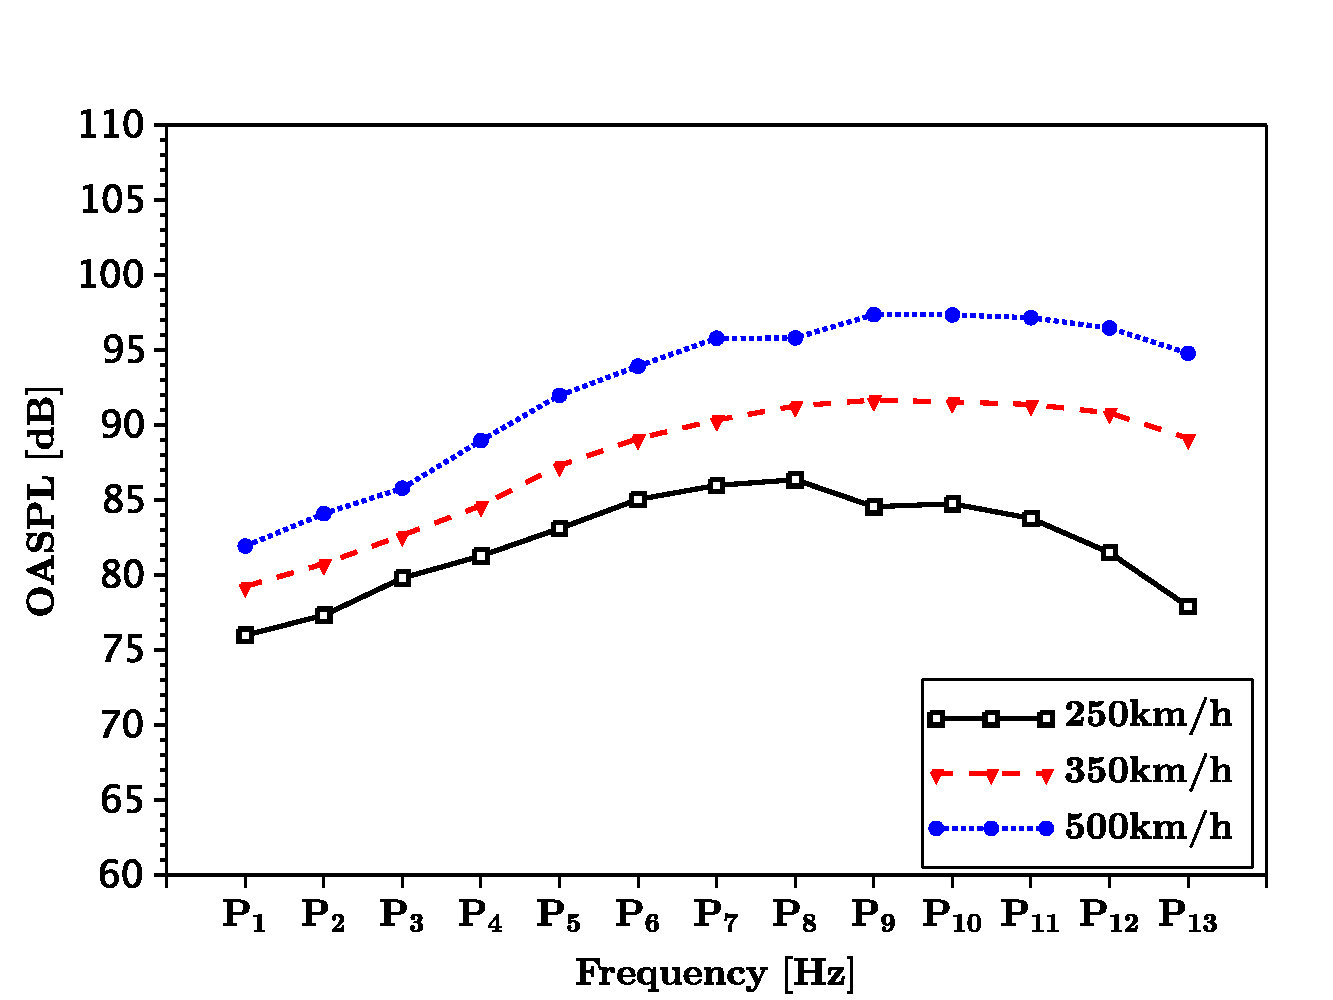
\includegraphics[width=\textwidth]{HC_OASPL_C}
                \caption{}
                \label{fig:HC_OASPL_C}
            \end{subfigure}%
            ~% add a small space
            \begin{subfigure}[b]{0.45\textwidth}
                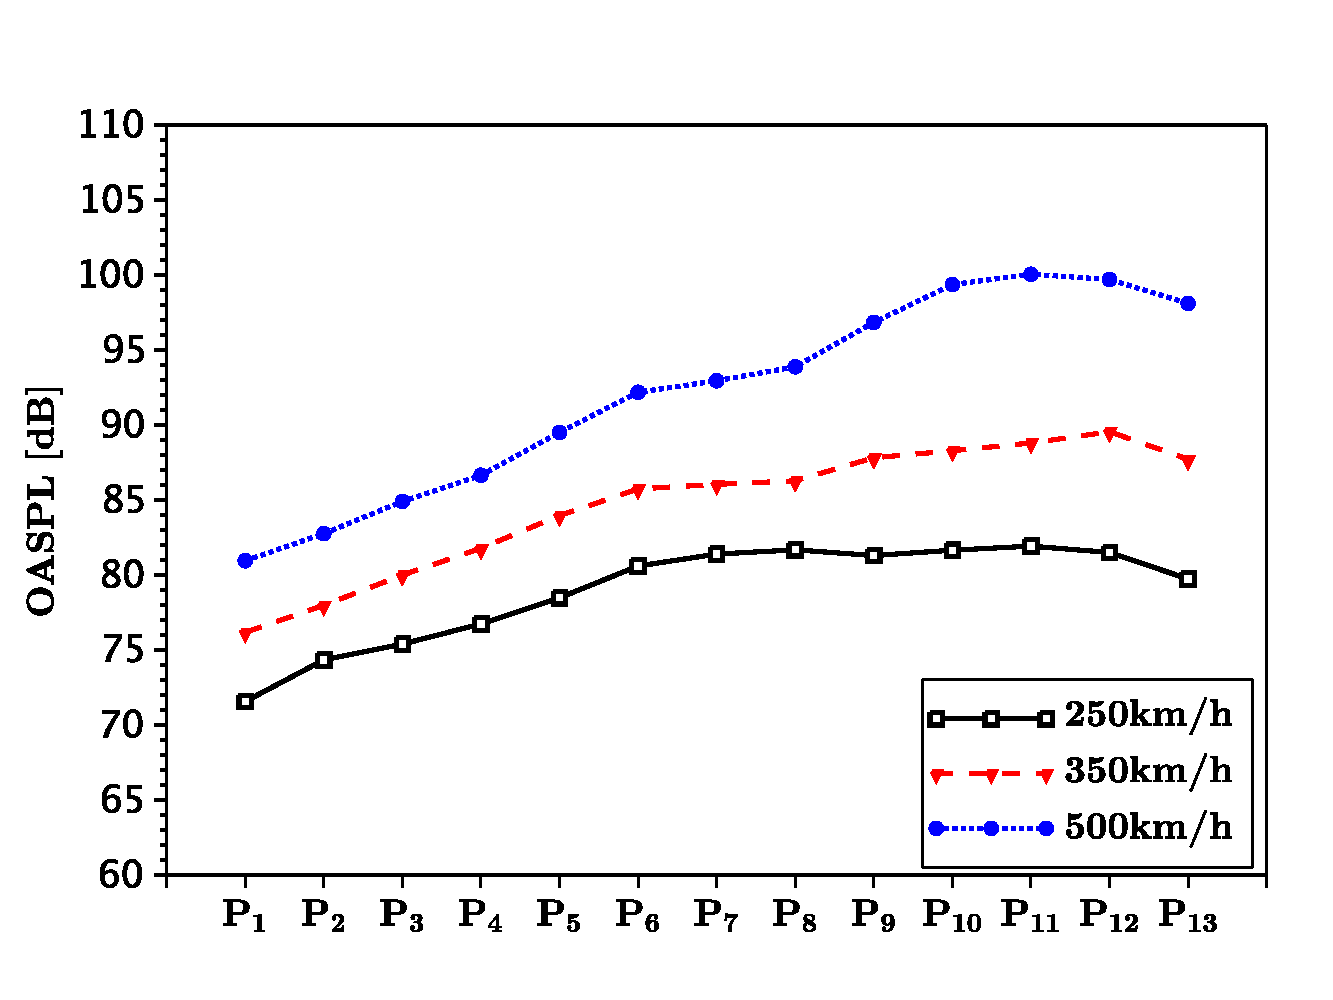
\includegraphics[width=\textwidth]{HC_OASPL_D}
                \caption{}
                \label{fig:HC_OASPL_D}
            \end{subfigure}%
            \caption{An Example for including multiple figures}
            \label{fig:HC_OASPL}
        \end{figure}
    \end{verbatim}
\end{center}
\begin{figure}[!htbp]
    \centering
    \begin{subfigure}[b]{0.45\textwidth}
        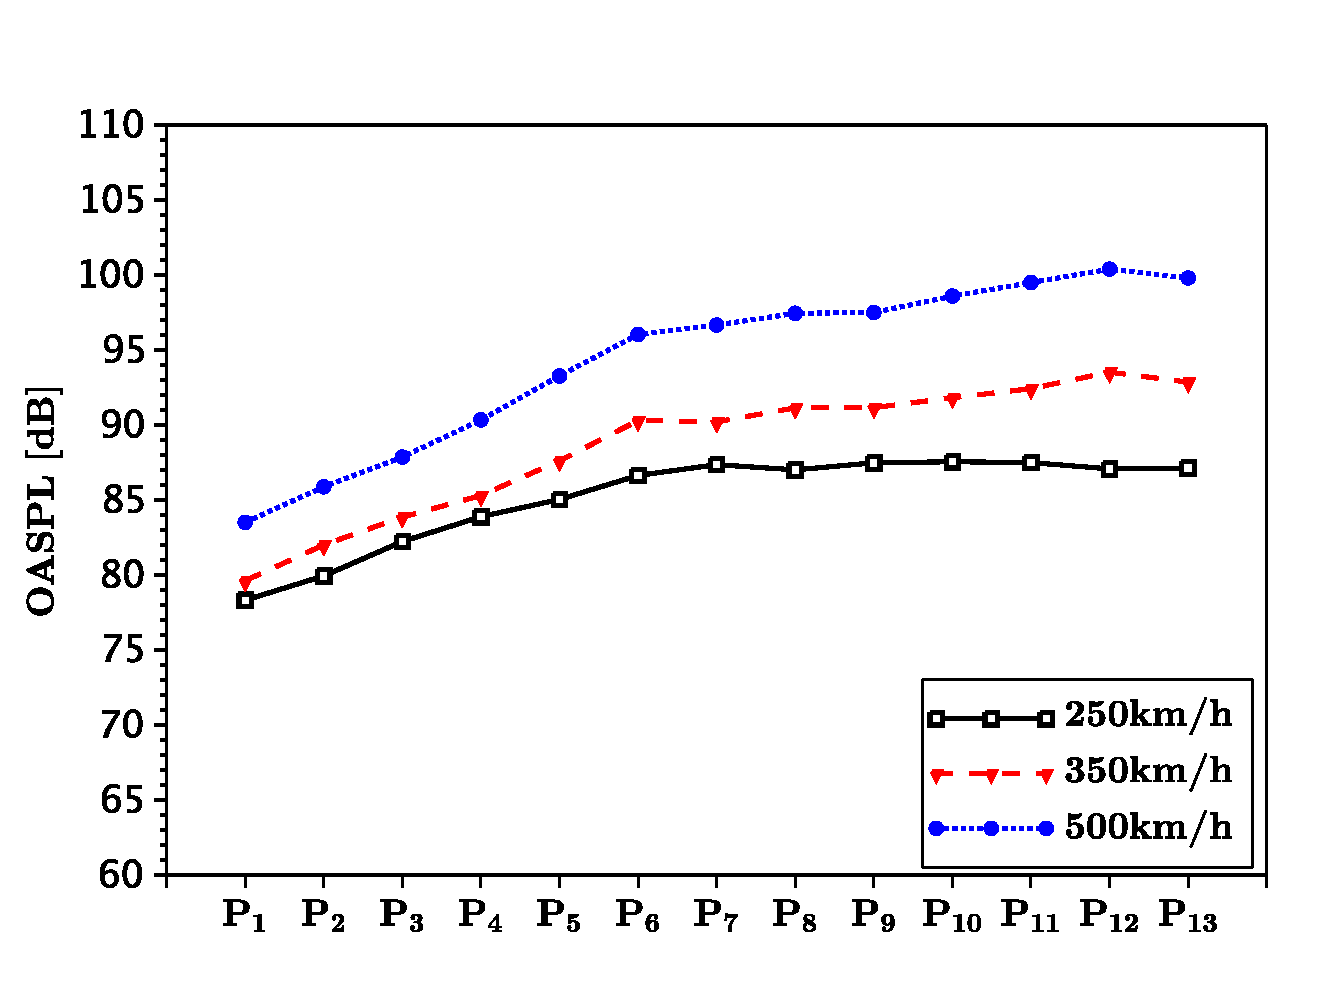
\includegraphics[width=\textwidth]{HC_OASPL_A}
        \caption{}
        \label{fig:HC_OASPL_A}
    \end{subfigure}%
    ~% add a small space
    \begin{subfigure}[b]{0.45\textwidth}
        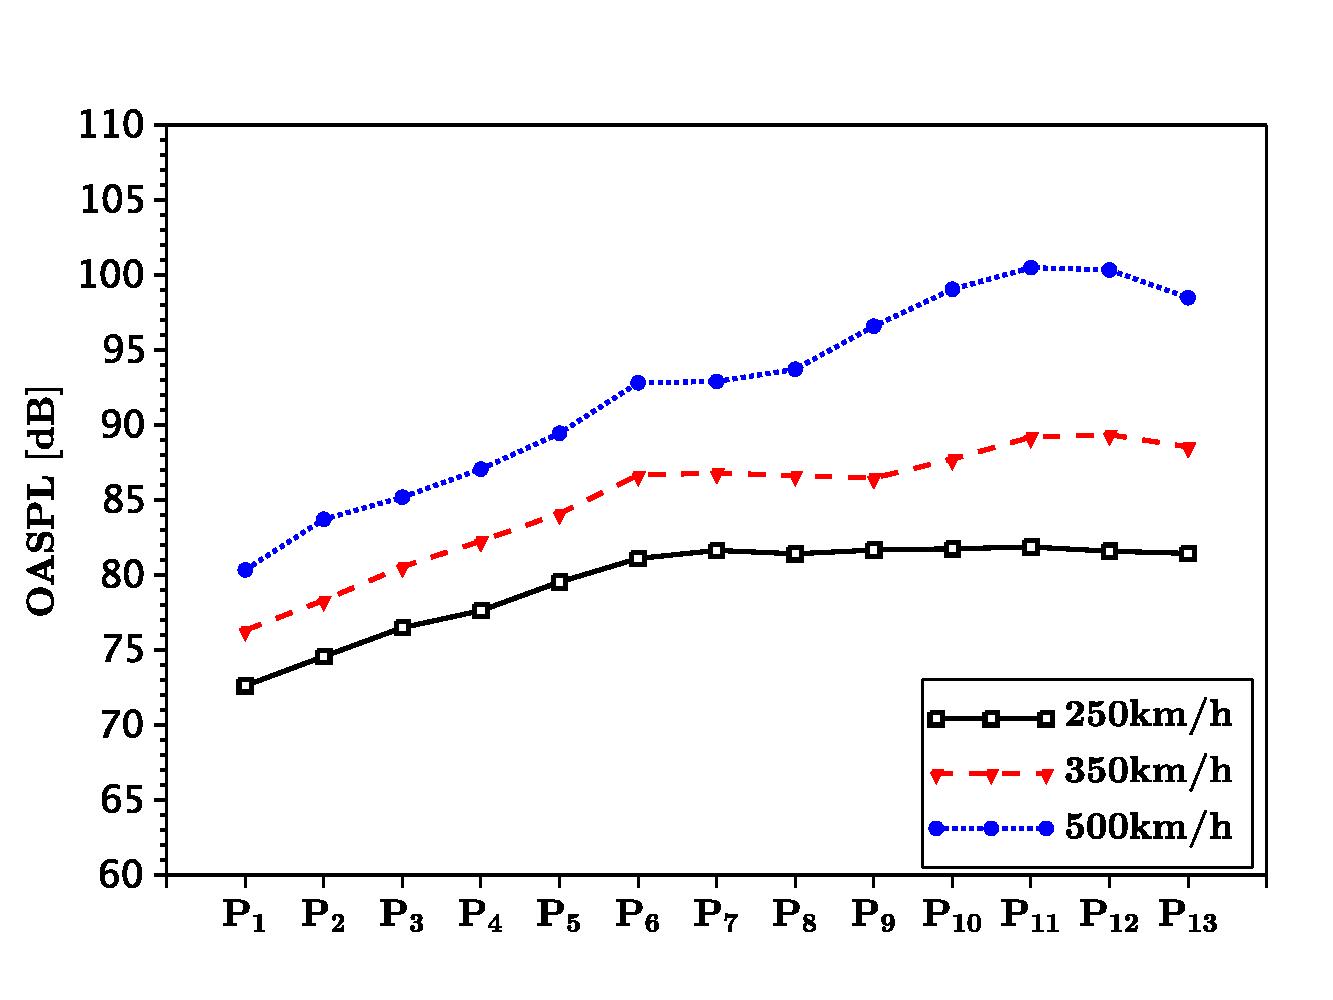
\includegraphics[width=\textwidth]{HC_OASPL_B}
        \caption{}
        \label{fig:HC_OASPL_B}
    \end{subfigure}%
    \\% change line
    \begin{subfigure}[b]{0.45\textwidth}
        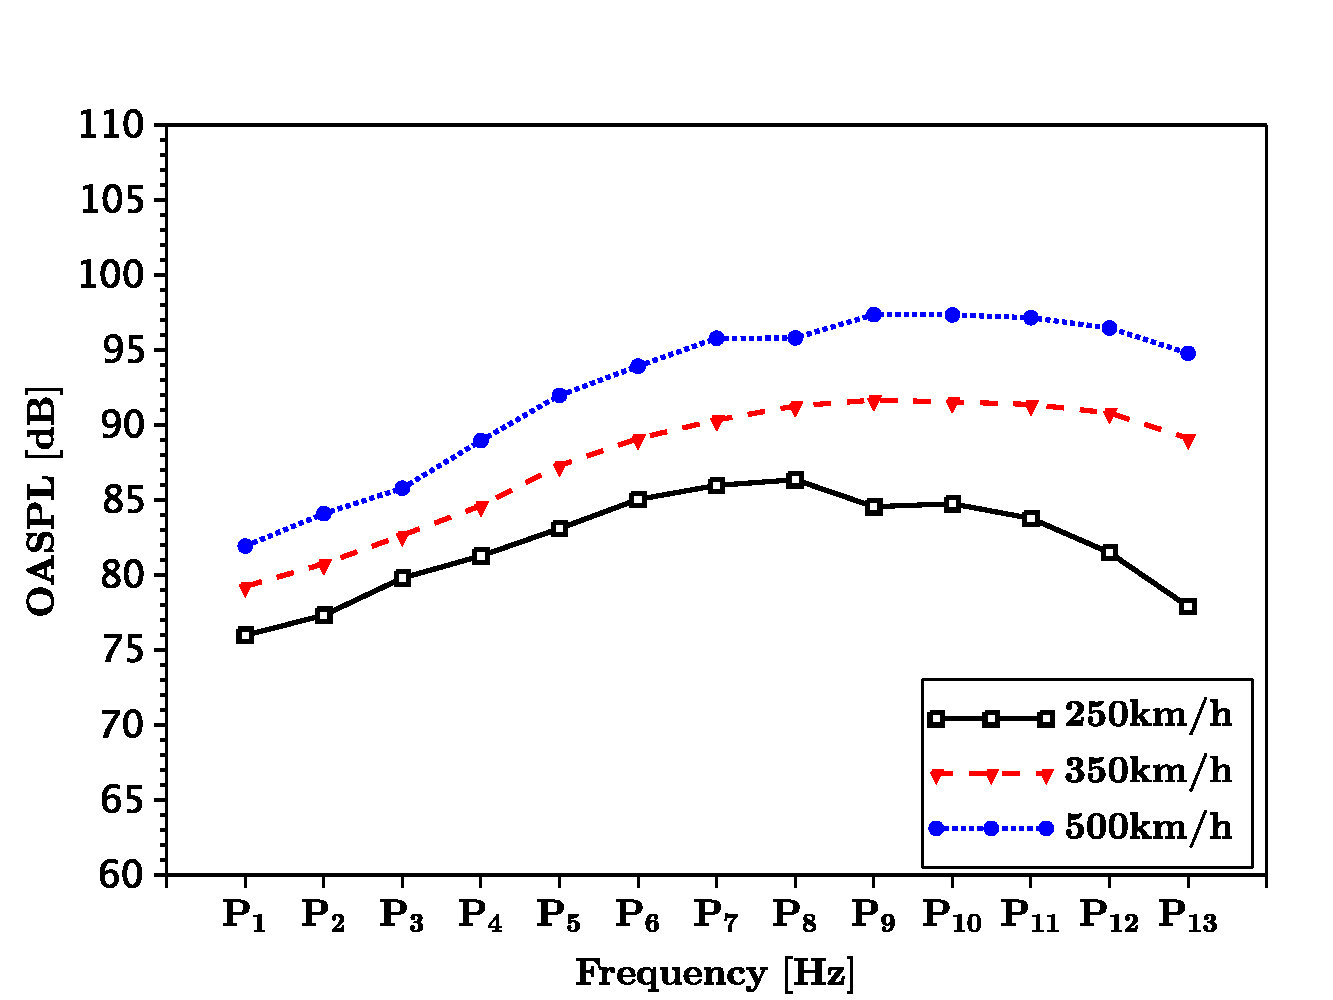
\includegraphics[width=\textwidth]{HC_OASPL_C}
        \caption{}
        \label{fig:HC_OASPL_C}
    \end{subfigure}%
    ~% add a small space
    \begin{subfigure}[b]{0.45\textwidth}
        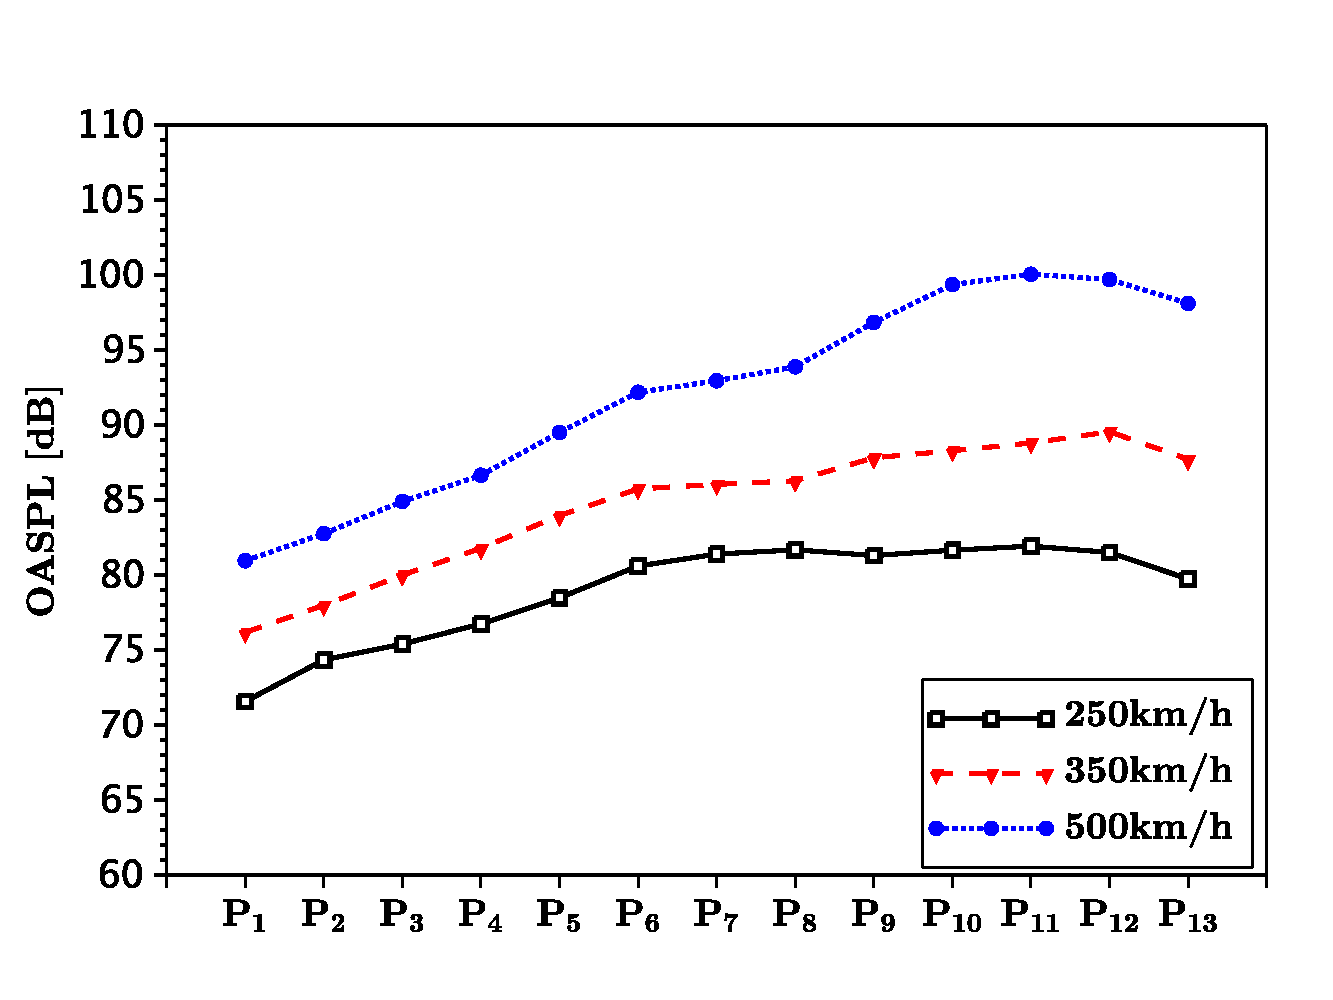
\includegraphics[width=\textwidth]{HC_OASPL_D}
        \caption{}
        \label{fig:HC_OASPL_D}
    \end{subfigure}%
    \caption{An Example for including multiple figures}
    \label{fig:HC_OASPL}
\end{figure}
% subsection Include Graphics (end)

\subsection{Include a citation} % (fold)
Suppose you are going to cite an article named "Document Preparation System", the procedures are:
\begin{itemize}
    \item Use Google Scholar search "Document Preparation System".
    \item Open "Cite" and choose "Import to Bibtex" under the target item.
    \item Copy the citation information of this article into the file "Myrefs.bib"
    \item Research dominant: cite this article by \verb+\citep{lamport1986document}+ like here \citep{lamport1986document}
    \item Citation dominant: cite this article by \verb+\citet{lamport1986document}+ like here \citet{lamport1986document}
    \item References list is generated automatically.
\end{itemize}
% subsection Include a citation (end)
\subsection{Generate nomenclature} % (fold)
In this template, a simple command for adding nomenclatures is provided. Therefore, packages for automatical nomenclature generation are not included. From my point of view, there is no need to use those packages and make things complicated. However, if you insist, there are a lot of available packages for creating nomenclatures. Recommended options are (Please Google the one you want to know):
\begin{itemize}
    \item listofsymbols
    \item nomencl
\end{itemize}

%%% ++++++++++++++++++++++++++++++++++++++++++++++++++++++++++++++++++++++++++++++++++
%
%%%%% --------------------------------------------------------------------------------
%%
%%%%*********************************Appendix*****************************************
%%
%% Some subordinate chapters.
\appendix%
\renewcommand{\thesection}{A.\arabic{section}}
\chapter{Appendix A: Python Scripts}
\label{appendix:a}
%\intotoc{Appendix A: Python Scripts}
\nopagebreak
\begin{small}
	
	\section{Capstan}
	\label{appendix:a0}
	\lstinputlisting[language=Python]{Capstan.py}
	\pagebreak	
	
	\section{ASME's BPVC VIII-1}
	\label{appendix:a1}
	\lstinputlisting[language=Python]{DivVIII1.py}
	\pagebreak
	
	\section{ASME's BPVC VIII-2}
	\label{appendix:a2}
	\lstinputlisting[language=Python]{DivVIII2.py}
	\pagebreak
	
	\section{EN 13445-3}
	\label{appendix:a3}
	\lstinputlisting[language=Python]{EN134453.py}

\end{small}

%%------------------------------------------------------------------------------------
\renewcommand{\thesection}{B.\arabic{section}}
\chapter{Appendix B: Excel Spreadsheet}
\label{appendix:b}

\vfill
\begin{center}
This page is left intentionally blank for insertion of Excel spreadsheet
\end{center}
\vfill

\includepdf[pages={1-2}]{Calcs/Uniform_p.pdf}

%%%------------------------------------------------------------------------------------
%\renewcommand{\thesection}{C.\arabic{section}}
%\chapter{Appendix C: FEA Results}
%\label{appendix:c}%
%%%%% --------------------------------------------------------------------------------
%%
%%%%********************************Backmatter****************************************
%%
%% Matters of Bibliography, Glossary, Index.
\backmatter
%%
%%% >>> Bibliography
%%
\bibliography{Myrefs}%
\intotoc{References}% add a corresponding item to the contents table and bookmark
%%
\end{document}
%%%%% --------------------------------------------------------------------------------
